\section{Product perspective}
\label{s:Product_perspective}%

\subsection{Class Diagram}
\label{ss:class_diagram}%
Here we provide the class diagram of our system and a brief description on some of the key aspects. The very first thing to explain is its logical split of the \textit{Static Analyzer} from the rest of the system, the reason for this is that we wanted to have a system that could be more \textit{flexible} than usual. The two logical parts can be implemented in the same tier or can also be split physically in terms of devices. What does not change is that when the STs set up github actions on their repository, the server that will be called when a commit is pushed is the \textbf{\textit{SA\_Server}}, which will do the necessary checks and then sends the results to the main server (\textbf{\textit{Results API}} has this purpose), where the score will be computed. Note that the Static Analyzer can be configured from the main server by using the provided APIs in \textbf{\textit{SA\_Configuration API}} (e.g., upload the test cases…). 
As asked by the assignment we distinguished two types of \textit{Users}, \textbf{\textit{Students}} and \textbf{\textit{Educators}}, in order to differentiate the features the platform offers to the two. The same concept is also applied to the participants of a battle, which does not distinguish a team from a single student; this is very useful when the battle finishes and the results have to be translated into the competition. The \textbf{\textit{NotificationHandler}} has the purpose of handling the notifications of the users and it provides the procedures to do just so.

\begin{center}
  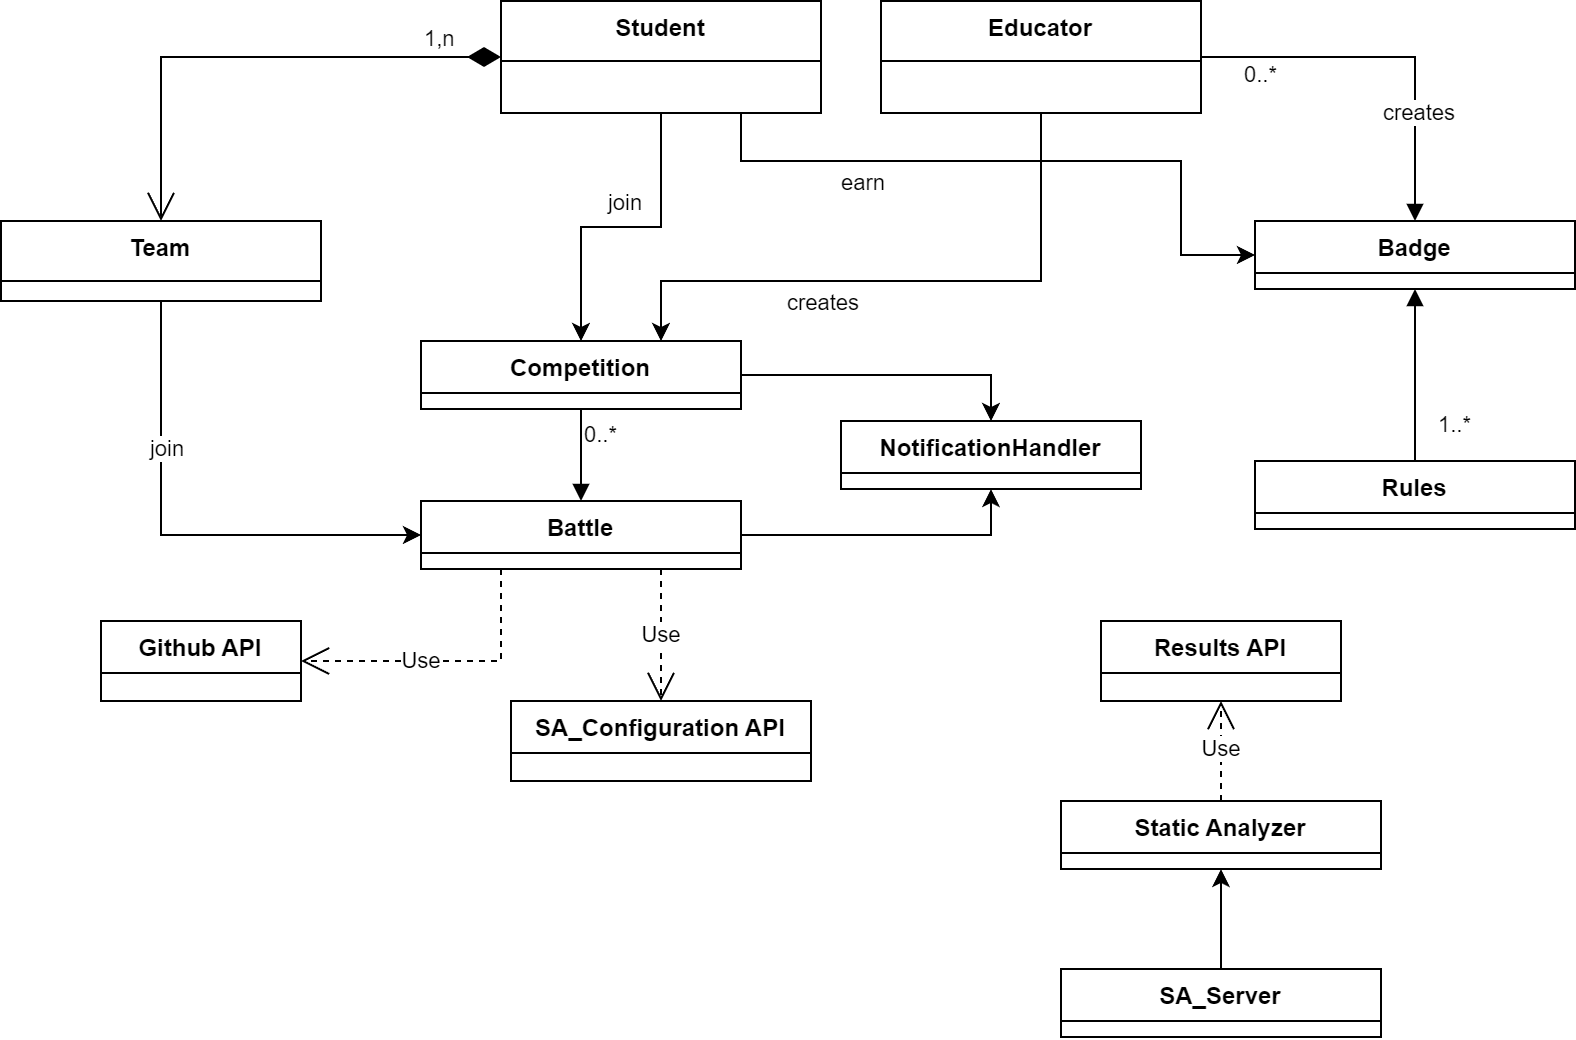
\includegraphics[width=\textwidth]{RASD_UML.png}
\end{center}

\subsection{State Diagrams}
\label{ss:state_diagrams}%

\subsection{Scenarios}
\label{ss:scenarios}%
\textbf{Scenario 1:} Professor Harry is a professor teaching at Politecnico di Milano together with professor Donald. Harry would like to encourage his students to study during the course, instead of having to study everything a few days before the exam. To do so he came up with the idea to create a challenge where the students can test their preparation and earn some extra points in the exam. While talking with other colleagues, Prof. Harry discovered CKB and he thought it was the perfect fit to implement his idea. The first thing he does is to go to the webpage of CKB and create an account by clicking the \textbf{\textit{Sign up}} button and providing some information about himself. Afterwards he is redirected to the home page of the platform where he can click the button \textbf{\textit{Create Competition}}, and finally he inserts the name of the competition and the subscription deadline. At this point he wants to invite his colleague Donald to manage the competition with him; since he is an ED in the competition he can click on \textbf{\textit{Invite Educator}} in the competition page, then provides the email of Donald's account, who will be part of the competition once he accepts the invite.


\textbf{Scenario 2:} Professor Harry is an ED of a competition, within which he wants to create a battle. To do so he enters the dashboard of the competition, clicks on the button \textbf{\textit{Create Battle}} and provides everything the platform needs: description, test cases, build automation scripts, deadlines, accepted sizes of groups. Marco, a ST who subscribed to the competition, received the notitication about the newly created battle via email. Outside of the platform Marco agreed with a couple of friends to participate in the battle together. Marco then goes on the competition page and finds the newly created battle, here he finds two buttons, \textbf{\textit{Participate as: 1. Loner 2. Team}}; he clicks the second button to participate as a team and invites his friends by providing the platform his friends' account email. Once Marco's friends accepted the invite the subscription to the battle will be automatically finalized by the platform.


\textbf{Scenario 3:} Professor Harry wants to give credit to the hardest working student, so while creating the competition he decided to create a new badge. The hardest working ST is the one that has written the highest amount of code lines among all the battles in the same competition. To implement this badge Prof. Harry must create a new variable \textbf{\textit{hardest\_worker}} and provide the code that defines how to compute the value of such variable. Some time after the specification of this new badge, a ST, participating in the competition and in the current battle, called Marco, pushes a commit to his repository. Since all students are supposed to setup \textit{GitHub Actions}, CKB is notified about Marco's commit, so it proceeds to run the required processes to calculate the new score, but also checks if Marco acquired new badges by checking their rules. Assuming that with the last commit Marco has now the most written lines of code, CKB assigns to him the \textit{hardest\_worker} badge.


\textbf{Scenario 4:} Marco and his team participated in a battle provided by Prof. Harry, one of the ED of the competition. Since the battle ends the next day, Marco wants to look at the partial rankings of the battle, so he goes on the page related to the battle and clicks on the \textit{Results} section, and sees his team at the bottom of the chart. Understandably, Marco's team resumes to work on the problem and they are able to commit a new version of their solution, which increased their placement in the partial rankings of the battle. The submission deadline now expired and the EDs now want to manually check the work of their STs to assign manually a score to each team; to do this Prof. Harry goes on the battle page and clicks on \textbf{\textit{Perform Manual check}}, which will redirect the ED to another page where he can inspect the source code of each team and give a score to each final work. Once this consolidation phase has been declared finished by an ED, CKB sends to all the STs subscribed to the competition a notification that the battle's results are available and the global scores of the competition have been updated.


\section{Product functions}
\label{s:Product_functions}%

\textbf{The ED can create a new competition} \\
The CKB allows the ED to create a new competition by clicking on the \textbf{\textit{Create Competition}} button on the home page, then providing the name of the competition and the subscription deadline.

The ED inside of the competition have the possibility to create a new battle by clicking on the \textbf{\textit{Create Battle}} button, where he can then insert the description, test cases and the solution. He can also set which aspects of the code he wants that CKB evaluate, such as the quality of the code, the number of lines of code, the security, the readability and the maintainability. Moreover he can select the minimum and maximum number of team components and the deadline for the submission.

Inside of each battle the ED can add badges by clicking on the \textbf{\textit{Add Badge}} button, where he can then insert the name of the badge, the description and the rules to assign the badge.

The ED can also invite other EDs to manage the competition with him by clicking on the \textbf{\textit{Invite Educator}} button and providing the email of the account of the ED he wants to invite. This will allow the colleague to change the settings of the competition and create new battles. \\

\textbf{The ST can participate in a competition} \\
The ST after logging in the platform can see the list of the competitions available, and can subscribe to them by clicking on the \textbf{\textit{Subscribe}} button. When the student clicks on the button he can choose to participate as a loner or as a team, in the latter case he has two possibilities: 
\begin{itemize}
  \item Create a new team by clicking on the \textbf{\textit{Create Team}} button, where he can then insert the name of the team and the email of the other STs he wants to invite. Once the other STs accepted the invite the subscription to the competition will be automatically finalized by the platform.
  \item Join an existing team by clicking on the \textbf{\textit{Join Team}} button. Once the team leader accepted the request,the ST will be added to the team.
\end{itemize}


After subscribing to a competition, the ST can see the list of the battles inside the competition and can subscribe to them by clicking on the \textbf{\textit{Subscribe}} button. When the student clicks on the button he can choose to participate as a loner or as a team, in the latter case he can invite other STs to participate in the battle with him by sending them an invite via email.

Inside the competition ST can also see the general ranking of the competition, which is updated after each battle. It is also possible to see the partial ranking of each battle he have partecipated in, which is updated after each submission. 

Another feature available to the ST is the possibility to see the list of the badges he earned, and the list of the badges he can earn with the corresponding rules. \\


\textbf{The CKB can evaluate the submissions} \\
The CKB is able to automatically evaluate the submissions of the STs by running the test cases provided by the EDs. Each new code submission made on the Github repository of the STs is notified to the CKB, which then runs the test cases on the code.

The test cases are run in a sandbox environment to prevent malicious code from damaging the system. The CKB is also able to run the build automation scripts provided by the EDs to check if the code compiles and if it satisfies the requirements. 

The code is evaluated also considering the quality of the sources by running static analysis tools on the code that considers the complexity of the code, the readability and the maintainability.

The CKB after performing all the checks assigns a score to the submission and updates the ranking of the battle and the competition. It also checks if the STs earned new badges by checking their rules and, in case, assigns them to the STs.

It is also possible for the ED managing the battle to manually evaluate the submissions by clicking on the \textbf{\textit{Perform Manual Check}} button on the battle page. This will redirect the ED to another page where he can inspect the source code of each team and give a score to each final work. Once this consolidation phase has been declared finished by an ED, CKB sends to all the STs subscribed to the competition a notification that the battle's results are available and the global scores of the competition have been updated.


\section{User characteristics}
\label{s:User_characteristics}%

The actors that are going to use the CKB system are:
\begin{itemize}
  \item \textbf{Educator (ED)}: an educator is a user that can create competitions and battles within competitions. He can set the parameters of the battles and the deadlines. He can also invite other educators to manage the competition with him.
  \item \textbf{Student (ST)}: a student is a user that can create teams and join battles as a team or individually. He can earn points and badges by partecipating in the competitions and battles.
\end{itemize}


\section{Assumptions, dependencies and constraints}
\label{s:Assumptions_dependencies_and_constraints}%

\begin{table}[H]
  \begin{tabular}{|l|l|}

    \hline
    \textbf{ID} & \textbf{Description}      \\
    \hline
    DA1 & ST owns a device able to connect to the internet \\
    \hline
    DA2 & ST owns a GitHub account \\
    \hline
    DA3 & ST has installed Git on his computer \\
    \hline
    DA4 & ST knows how to use Git \\
    \hline
    DA5 & ED knows how to use Git \\
    \hline
    DA6 & ED owns a device able to connect to the internet \\
    \hline
    DA7 & ED writes correct tests \\ 
    \hline
    DA8 & ED correctly evaluates the final source code of a T \\
    \hline
    DA9 & GitHub permits automatic push to a repository \\
    \hline
    DA10 & GitHub permits automatically pull from a repository \\
    \hline
    DA11 & ST knows the usernames of other STs they want to invite to a T  \\
    \hline
    DA12 & STs has an internet connection \\
    \hline
    DA13 & ED has an internet connection \\
    \hline
    DA14 & ST writes code only with languages that are treatable by the platform \\
    \hline
    DA15 & ED knows the email of the other EDs he wants to invite to manage a competition \\
    \hline
    DA16 & ED writes the correct badge’ rules \\
    \hline

    
  \end{tabular}
  \caption{List of the domain assumption}
  \label{tab:domainAssumption}
\end{table}
